	\documentclass[a4paper,twoside,11pt]{article}
\usepackage{a4wide,graphicx,fancyhdr,amsmath,amssymb,float,longtable,chronology,caption,subcaption,appendix}
\usepackage{algorithmic}
\usepackage{hyperref}
\usepackage{listings}
\usepackage{url}
\usepackage{pgffor}
\usepackage{color}

%----------------------- Macros and Definitions --------------------------

\definecolor{mygreen}{rgb}{0,0.6,0}
\definecolor{mygray}{rgb}{0.5,0.5,0.5}
\definecolor{mymauve}{rgb}{0.58,0,0.82}

\lstset{ %
  backgroundcolor=\color{white},   % choose the background color; you must add \usepackage{color} or \usepackage{xcolor}
  basicstyle=\footnotesize,        % the size of the fonts that are used for the code
  breakatwhitespace=false,         % sets if automatic breaks should only happen at whitespace
  breaklines=true,                 % sets automatic line breaking
  captionpos=b,                    % sets the caption-position to bottom
  commentstyle=\color{mygreen},    % comment style
  deletekeywords={...},            % if you want to delete keywords from the given language
  escapeinside={\%*}{*)},          % if you want to add LaTeX within your code
  extendedchars=true,              % lets you use non-ASCII characters; for 8-bits encodings only, does not work with UTF-8
  frame=single,	                   % adds a frame around the code
  keepspaces=true,                 % keeps spaces in text, useful for keeping indentation of code (possibly needs columns=flexible)
  keywordstyle=\color{blue},       % keyword style
 % language=mcrl2,                 % the language of the code
  otherkeywords={*,...},           % if you want to add more keywords to the set
  numbers=left,                    % where to put the line-numbers; possible values are (none, left, right)
  numbersep=5pt,                   % how far the line-numbers are from the code
  numberstyle=\tiny\color{mygray}, % the style that is used for the line-numbers
  rulecolor=\color{black},         % if not set, the frame-color may be changed on line-breaks within not-black text (e.g. comments (green here))
  showspaces=false,                % show spaces everywhere adding particular underscores; it overrides 'showstringspaces'
  showstringspaces=false,          % underline spaces within strings only
  showtabs=false,                  % show tabs within strings adding particular underscores
  stepnumber=2,                    % the step between two line-numbers. If it's 1, each line will be numbered
  stringstyle=\color{mymauve},     % string literal style
  tabsize=2,	                   % sets default tabsize to 2 spaces
 % title=\lstname                   % show the filename of files included with \lstinputlisting; also try caption instead of title
}


\setlength\headheight{20pt}
\addtolength\topmargin{-10pt}
\addtolength\footskip{20pt}

\newcommand{\N}{\mathbb{N}}
\newcommand{\ch}{\mathcal{CH}}
\everymath{\displaystyle}
\newcommand{\define}[2]{\noindent{\bf #1}}
\newcommand{\scg}{Generic Language Technology}

\newcommand{\action}[2]{{\tt #1(#2)}}
\newcommand{\todo}[1]{{\color{red}#1}}

\fancypagestyle{plain}{%
	\fancyhf{}
	\fancyhead[LO,RE]{\sffamily\bfseries\large Technische Universiteit Eindhoven}
	\fancyhead[RO,LE]{\sffamily\bfseries\large 2IMP20 \scg}
	\fancyfoot[LO,RE]{\sffamily\bfseries\large Department of Mathematics and Computer Science}
	\fancyfoot[RO,LE]{\sffamily\bfseries\thepage}
	\renewcommand{\headrulewidth}{0pt}
	\renewcommand{\footrulewidth}{0pt}
}

\pagestyle{fancy}
\fancyhf{}
\fancyhead[RO,LE]{\sffamily\bfseries\large Technische Universiteit Eindhoven}
\fancyhead[LO,RE]{\sffamily\bfseries\large 2IMP20 - Generic Language Technology}
\fancyfoot[LO,RE]{\sffamily\bfseries\large Department of Mathematics and Computer Science}
\fancyfoot[RO,LE]{\sffamily\bfseries\thepage}
\renewcommand{\headrulewidth}{1pt}
\renewcommand{\footrulewidth}{0pt}


%-------------------------------- Title ----------------------------------

\title{\sffamily\bfseries 2IMP20 \scg\ - Assignment 3\\ A Domain-Specific Language for Lego Vehicles}
\author{Ruud Andriessen \qquad Student number: 0770663\\{\tt r.andriessen@student.tue.nl}\\\\ Hein van Beers \qquad Student number: 0765658 \\{\tt h.a.v.beers@student.tue.nl}}

\date{\today}

\allowdisplaybreaks

%--------------------------------- Text ----------------------------------

\begin{document}
\maketitle
\section{Introduction}
In this paper we will briefly discuss the decisions we made when designing the metamodel for the platoon language.

\section{Design decisions for the Platoon model}
Just like for the BoundingBox language, we created a \textit{World} class that has, as its children, several references to other classes. A \textit{World} can have a reference to one instance of the \textit{Platoon} class, one instance of the \textit{Route} class and a reference to an instance of the \textit{Constraints} class.\\

Since a platoon is defined to have a single leading vehicle and zero or more follow vehicles, we implemented the \textit{Platoon} class, such that it has a reference to a single instance of a \textit{LeadingVehicle} and zero or more references to instances of the \textit{FollowVehicle} class.\\

A route is specified to consist of at least one command and we should be able to refer to each route separately. This is why we modelled the \textit{Route} class to have a reference to one or more instances of the \textit{Command} class and an attribute \textit{id} of the type \textit{String}, which can be used as an identifier.\\

The \textit{Constraints} class has zero or more references to instances of the \textit{Constraint} class, since it represents the list of constraints that the platoon should satisfy. The \textit{Constraint} class is used as a super type for the \textit{HeadwayConstraint} class.\\

The \textit{Vehicle} class is an abstract class containing a single attribute \textit{id} of the type \textit{String}, which is used as a unique identifier for a vehicle.\\

A \textit{FollowVehicle} has the \textit{Vehicle} class as its super type and contains a reference  to a single instance of \textit{Vehicle}, which is called \textit{FrontRunner} and refers to the identifier of the vehicle in front of this \textit{FollowVehicle}.\\

A \textit{LeadingVehicle} also has the \textit{Vehicle} class as its super type and contains a reference to a single instance of \textit{Route}, which refers to the route that the \textit{LeadingVehicle} needs to follow.\\

The \textit{Command} class is an abstract class and is used as a super type for the \textit{ForwardCommand} class and the \textit{TurnCommand} class.\\

Each \textit{ForwardCommand} has a single attribute, which is used to identify the distance that the vehicle needs to go forward, when executing this command.\\

Each \textit{TurnCommand} has a reference to the \textit{Direction} class, which is used to identify the direction in which it needs to turn, when executing this command.\\

The \textit{Direction} class is an abstract class and is used as a super type for the \textit{Left} class and the \textit{Right} class, which are used to indicate that the vehicle needs to turn left or right, respectively.\\

The \textit{HeadwayConstraint} class has the \textit{Constraint} class as its super type and it contains two attributes of the type \textit{Int}. These attributes (\textit{min} and \textit{max}) are used to indicate the minimal and maximal distance in between which the vehicle needs to stay compared to the vehicle in front of him.\\


\begin{figure}[h]
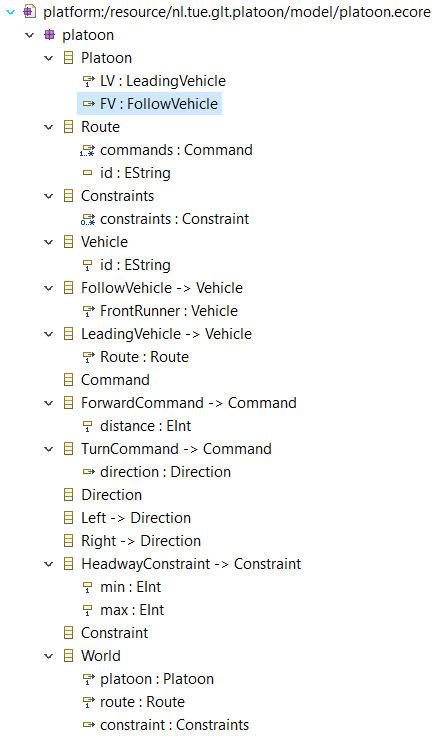
\includegraphics{platoon.PNG}
\caption{Visualization of the platoon ecore model.}
\label{platoon-ecore}
\end{figure}

\end{document}
